\documentclass[12pt]{article}
\usepackage{amsmath}  % Math
\usepackage{amssymb}  % Symbols
\usepackage{graphicx} % Images
\usepackage[utf8]{inputenc}
\usepackage[T1]{fontenc}
\usepackage[margin=1in]{geometry}
\usepackage[spanish]{babel}
\usepackage{transparent}
\usepackage{eso-pic}
\usepackage{xcolor}
\usepackage{subcaption} % For subfigures

\graphicspath{{images/}} % Path to images
\newcommand\BackgroundPic{
    \put(0,0){
        \parbox[b][\paperheight]{\paperwidth}{
            \vfill
            \centering
            \transparent{0.1}
\includegraphics[width=\paperwidth]{logo} % your image
            \vfill
        }
    }
}


\title{Informe Negocio Empanadas: \\
\textit{Las Empanadas Hermanas}} % Title of the report
  \author{Autores: Felipe Colli, Juan Gonzalez, Bastián Ortiz y Javier Robles \thanks{Instituto Nacional General José Miguel Carrera} \\
  Curso: \textit{4°H}, Profesor: \textit{Carlos Morales}} % Add your names and course
  \date{30 de mayo de 2025} % Fecha de Entrega
\AddToShipoutPicture{\BackgroundPic} % Add background image

\begin{document}

\maketitle
%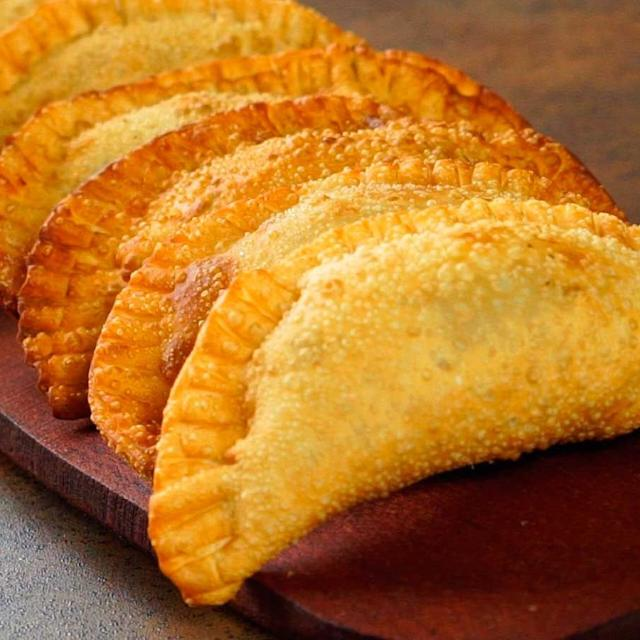
\includegraphics[width=0.95\textwidth]{empanadas} % Logo of the school
\newpage

\tableofcontents
\newpage

\section{Resumen} % Aprox 1/3 de Pagina
% Content for Resumen
\newpage



\section{Introducción} % Max 1 pagina
El presente informe tiene como objetivo presentar el negocio de empanadas "Empanadas de Juancho", un emprendimiento que busca ofrecer empanadas de alta calidad. A través de este documento, se detallarán los aspectos clave del negocio, incluyendo su propuesta de valor, mercado objetivo y proyecciones financieras. \\


Dentro de las proyeciones financieras, se contempla un análisis de costos y precios, así como una estimación de las ganancias esperadas. El negocio se enfoca en la producción y venta de 3 tamaños de empanadas de queso, con un énfasis en la calidad de los ingredientes y la satisfacción del cliente, sin olvidar el marco legal regulatorio, por lo cual este negocio no sera un frente para lavado de activos, evasion de impuestos, generacion de facturas ideologicamnete falsas, o la venta de drogas. \\ % Referencia a Breking Bad y Los Pollos Hermanos


\subsection{Objetivos del Negocio:}
\begin{enumerate}
    \item \textbf{Propuesta de Valor:} Ofrecer empanadas de alta calidad, elaboradas con ingredientes frescos y locales, destacando la variedad de sabores y la atención al cliente.
    \item \textbf{Mercado Objetivo:} El negocio se enfocará en consumidores locales que valoran la calidad y la autenticidad en sus alimentos, así como en aquellos que buscan opciones convenientes y deliciosas para sus comidas diarias.
    \item \textbf{Proyecciones Financieras:} Se espera que el negocio genere ingresos sostenibles a través de la venta de empanadas, con un enfoque en la rentabilidad a largo plazo. Las proyecciones incluirán un análisis detallado de costos, precios y ganancias esperadas.
    \item \textbf{Análisis de Costos y Precios:} Se realizará un estudio exhaustivo de los costos asociados con la producción y venta de empanadas, sin incluir mano de obra y gastos operativos. Además, se establecerán precios competitivos que reflejen la calidad del producto y permitan un margen de ganancia adecuado.
    \item \textbf{Estudio de Mercado:} Se llevará a cabo un análisis del mercado local para identificar las tendencias y preferencias de los consumidores, así como la competencia existente en el sector de alimentos. Esto permitirá ajustar la estrategia del negocio para maximizar su éxito.
    \item \textbf{Marco Legal:} El negocio se compromete a operar dentro del marco legal regulatorio, asegurando que todas las operaciones sean transparentes y cumplan con las normativas vigentes. Esto incluye la obtención de licencias necesarias y el cumplimiento de las normativas de seguridad alimentaria.
    \item \textbf{Viabilidad del Negocio:} Se evaluará la viabilidad del negocio a través de un análisis financiero detallado, que incluirá proyecciones de ingresos, costos y ganancias. Esto permitirá determinar si el negocio es sostenible a largo plazo y si puede generar un retorno adecuado sobre la inversión inicial.
\end{enumerate}

\newpage



\section{Desarrollo} % 2 - 5 paginas

\subsection{Tabla de Costos Ingredientes}

\begin{table}[h!]
    \centering
    \begin{tabular}{|| c | c | c | c||} 
        \hline
    \textbf{Distribuidor} & Unidades & \textbf{Costo} & \textbf{Costo 100 Unidades} \\ [0.5ex]
        \hline\hline
        \multicolumn{4}{||c||}{\textbf{Masa Prehecha Grande}} \\ [0.5ex] \hline \hline
        El Palacio de las Empanadas & 20 Un & \$4100 & \$20500 \\ \hline
        Masas Mi Tierra & 25 Un & \$8000 & \$31000 \\ \hline
        Alimentos La Kosa & 20 Un & \$4200 & \$21000 \\ [1ex] \hline \hline

        \multicolumn{3}{||c||}{\textbf{Huevos}} & \textbf{Costo por Docena} \\ [0.5ex] \hline \hline
        El Don Huevo & 180 Un & \$39500 & \$2633 \\ \hline
        Huevos La Montaña Pelluhue & 180 Un & \$43990 & \$2932 \\ \hline
        AgricoVial & 180 Un & \$41600 & \$2773 \\ [1ex] \hline \hline

        \multicolumn{3}{||c|}{\textbf{Camaron}} & \textbf{Costo por KG} \\ [0.5ex] \hline \hline
        Distribuidora GK & 10 KG & \$48900 & \$4890 \\ \hline
        Comercial Oceanica & 10 KG & \$55800 & \$5580 \\ \hline
        Del Origen & 10 KG & \$48700 & \$4870 \\ [1ex] \hline \hline

        \multicolumn{3}{||c|}{\textbf{Carne Molida}} & \textbf{Costo por KG} \\ [0.5ex] \hline \hline % Added Costo por KG header for consistency
        Central Mayorista & 500 G & \$2590 & \$5080 \\ \hline 
        Unimarc & 1 KG & \$4990 & \$4990 \\ \hline 
        El Paiquito & 250 G & \$1090 & \$4360 \\ [1ex] \hline \hline


        \multicolumn{3}{||c|}{\textbf{Queso}} & \textbf{Costo por KG} \\ [0.5ex] \hline \hline % Added Costo por KG header
        Distribuidora Santiago & 1 KG & \$9580 & \$9580 \\ \hline
        Distribuidora Nueva de Matte & 1 KG & \$6940 & \$6940 \\ \hline
        Mayorista 10 & 1 KG & \$9160 & \$9160 \\ [1ex] \hline \hline

        \multicolumn{3}{||c|}{\textbf{Cebolla}} & \textbf{Costo por KG} \\ [0.5ex] \hline \hline % Added Costo por KG header
        Santiago Natural Foods & 14 KG & \$10990 & \$785 \\ \hline
        Distribuidora Frest & 10 KG & \$9990 & \$990 \\ \hline
        Lider & 1 KG & \$1195 & \$1195 \\ [1ex] \hline \hline

        \multicolumn{3}{||c|}{\textbf{Aceite}} & \textbf{Costo por Litro} \\ [0.5ex] \hline \hline
        ProsudMarket & 18 L & \$39614 & \$2200.77 \\ \hline
        Central Mayorista & 13.5 L & \$22200 & \$1644.44 \\ \hline
        Distribuidora Sabatini & 5L & \$9296 & \$1859.20 \\ [1ex] \hline \hline

    \end{tabular}
    \caption{Tabla de Costos de Ingredientes}
    \label{tab:costos_ingredientes}
\end{table}


\subsection{Cotizaciones Ingredientes}
    %\subsubsection{Masa Prehecha}
        \begin{figure}[h!] % Use [h!] or [htbp] for better float placement
            \centering % Center the content of the figure
            \begin{subfigure}{0.4\textwidth}
                \centering
                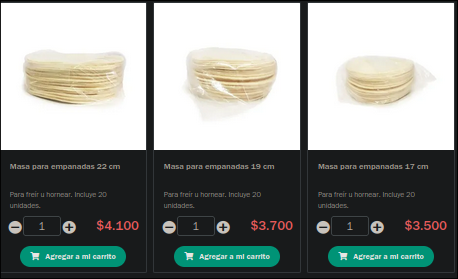
\includegraphics[width=0.9\linewidth]{palaci} % Removed space before ]
                \caption{Palacio de las Empanadas}
                \label{fig:palacio}
            \end{subfigure}
            \hfill % Add some space between subfigures
            \begin{subfigure}{0.4\textwidth}
                \centering
                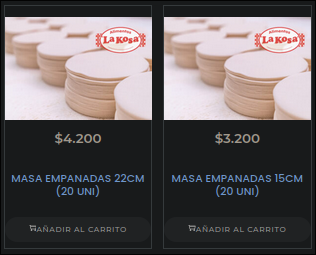
\includegraphics[width=0.9\linewidth]{kosa} % Removed space before ]
                \caption{Alimentos La Kosa}
                \label{fig:kosa}
            \end{subfigure}
            \caption{Cotizaciones de Distribuidores de Masa Prehecha}
            \label{fig:cotizaciones_masas}
        \end{figure} % END OF THIS FIGURE

    %\subsubsection{Huevos}
        \begin{figure}[h!] % START A NEW FIGURE
            \centering
            \begin{subfigure}{0.35\textwidth}
                \centering
                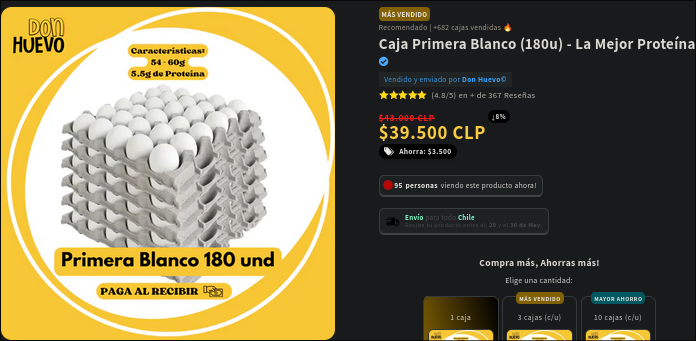
\includegraphics[width=0.9\linewidth]{donhuevo} % Removed space before ]
                \caption{El Don Huevo}
                \label{fig:don_huevo}
            \end{subfigure}
            \hfill
            \begin{subfigure}{0.4\textwidth}
                \centering
                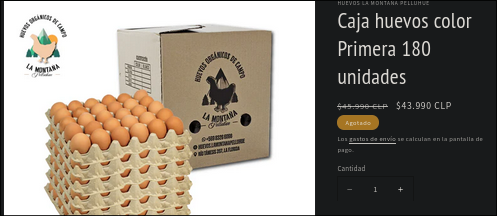
\includegraphics[width=0.9\linewidth]{montan1} % Removed space before ]
                \caption{Huevos La Montaña Pelluhue}
                \label{fig:huevos_montaña}
            \end{subfigure}
            \caption{Cotizaciones de Distribuidores de Huevos}
            \label{fig:cotizaciones_huevos}
        \end{figure} % END OF THIS FIGURE

    %\subsubsection{Camaron}
        \begin{figure}[h!] % START A NEW FIGURE
            \centering
            \begin{subfigure}{0.4\textwidth}
                \centering
                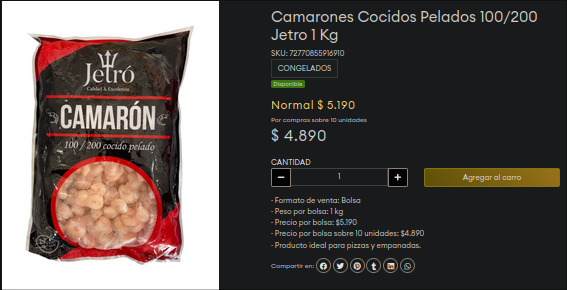
\includegraphics[width=0.9\linewidth]{gk} % Removed space before ]
                \caption{Distribuidora GK}
                \label{fig:distribuidora_gk}
            \end{subfigure}
            \hfill
            \begin{subfigure}{0.35\textwidth}
                \centering
                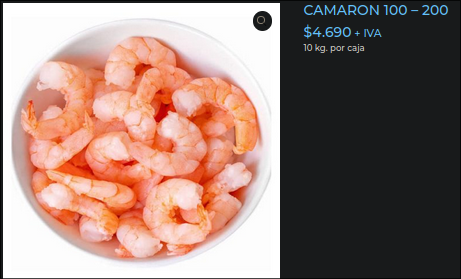
\includegraphics[width=0.9\linewidth]{oceanic} % Removed space before ]
                \caption{Comercial Oceanica}
                \label{fig:comercial_oceanica}
            \end{subfigure}
            \caption{Cotizaciones de Distribuidores de Camarón}
            \label{fig:cotizaciones_camaron}
        \end{figure} % END OF THIS FIGURE
        %\newpage % You can uncomment this if you specifically want a page break here

    %\subsubsection{Carne Molida}
        \begin{figure}[h!] % START A NEW FIGURE
            \centering
            \begin{subfigure}{0.45\textwidth}
                \centering
                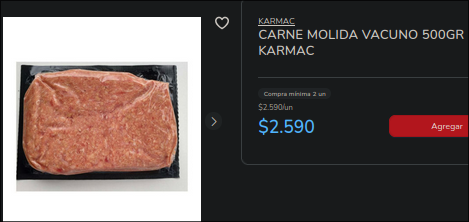
\includegraphics[width=0.9\linewidth]{central} % Removed space before ]
                \caption{Central Mayorista}
                \label{fig:central_mayorista}
            \end{subfigure}
            \hfill
            \begin{subfigure}{0.45\textwidth}
                \centering
                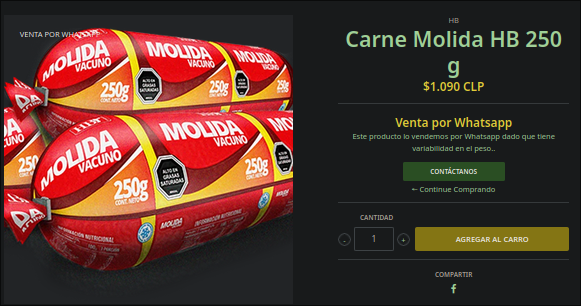
\includegraphics[width=0.9\linewidth]{paiquito} % Removed space before ]
                \caption{Paiquito}
                \label{fig:unimarc} % Consider if fig:paiquito is a more suitable label
            \end{subfigure}
            \caption{Cotizaciones de Distribuidores de Carne Molida}
            \label{fig:cotizaciones_carne_molida}
        \end{figure} % END OF THIS FIGURE

    %\subsubsection{Queso}
        \begin{figure}[h!] % START A NEW FIGURE
            \centering
            \begin{subfigure}{0.45\textwidth}
                \centering
                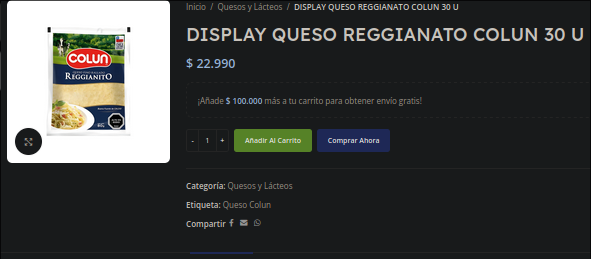
\includegraphics[width=0.9\linewidth]{santiago} % Removed space before ]
                \caption{Distribuidora Santiago}
                \label{fig:distribuidora_santiago}
            \end{subfigure}
            \hfill
            \begin{subfigure}{0.45\textwidth}
                \centering
                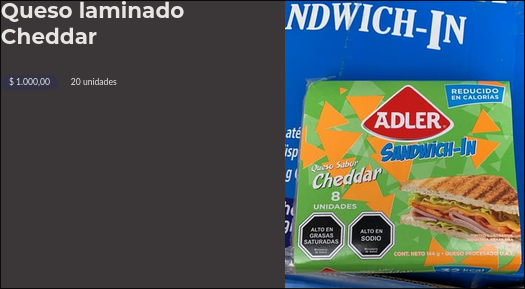
\includegraphics[width=0.9\linewidth]{nueva} % Removed space before ]
                \caption{Distribuidora Nueva de Matte}
                \label{fig:distribuidora_nueva_de_matte}
            \end{subfigure}
            \caption{Cotizaciones de Distribuidores de Queso}
            \label{fig:cotizaciones_queso}
        \end{figure} % END OF THIS FIGURE

    %\subsubsection{Cebolla}
        \begin{figure}[h!] % START A NEW FIGURE
            \centering
            \begin{subfigure}{0.4\textwidth}
                \centering
                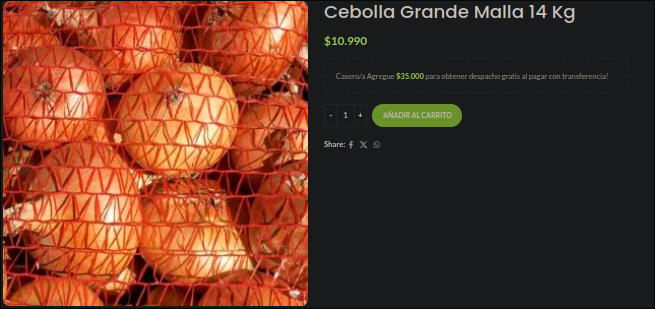
\includegraphics[width=0.9\linewidth]{nat} % Removed space before ]
                \caption{Santiago Natural Foods}
                \label{fig:santiago_natural_foods}
            \end{subfigure}
            \hfill
            \begin{subfigure}{0.45\textwidth}
                \centering
                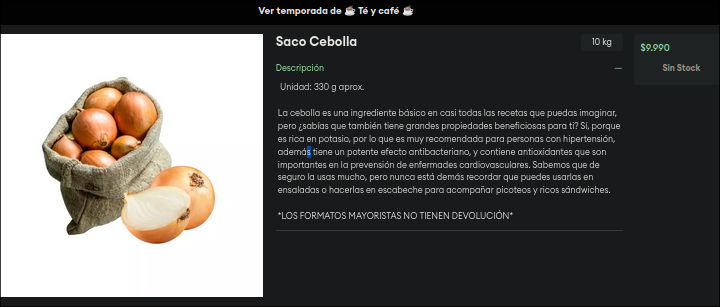
\includegraphics[width=0.9\linewidth]{fres} % Removed space before ]
                \caption{Distribuidora Frest}
                \label{fig:distribuidora_frest}
            \end{subfigure}
            \caption{Cotizaciones de Distribuidores de Cebolla}
            \label{fig:cotizaciones_cebolla}
        \end{figure} % END OF THIS FIGURE

    %\subsubsection{Aceite}
        \begin{figure}[h!] % START A NEW FIGURE
            \centering
            \begin{subfigure}{0.45\textwidth}
                \centering
                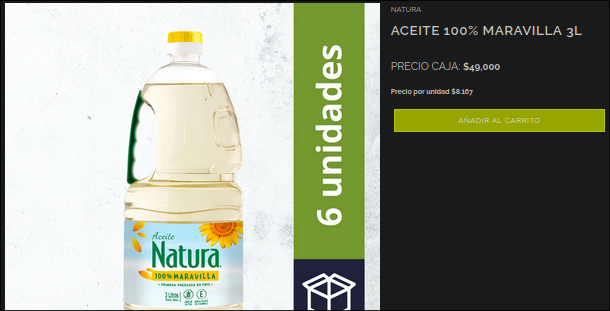
\includegraphics[width=0.9\linewidth]{prosud} % Removed space before ]
                \caption{ProsudMarket}
                \label{fig:prosudmarket}
            \end{subfigure}
            \hfill
            \begin{subfigure}{0.45\textwidth}
                \centering
                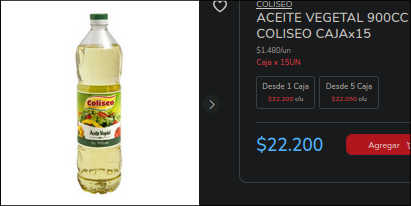
\includegraphics[width=0.9\linewidth]{aceite} % Removed space before ]
                \caption{Central Mayorista}
                \label{fig:central_mayorista_aceite}
            \end{subfigure}
            \caption{Cotizaciones de Distribuidores de Aceite}
            \label{fig:cotizaciones_aceite}
        \end{figure} % END OF THIS FIGURE
        
        \newpage % This newpage was already here, affecting layout before Conclusiones


\section{Conclusiones} % Max 1 pagina
% Content for Conclusiones


\end{document}
